%
% main.tex -- Paper zum Thema <maxwell>
%
% (c) 2020 Autor, OST Ostschweizer Fachhochschule
%
% !TEX root = ../../buch.tex
% !TEX encoding = UTF-8
%
\chapter{Vierdimensionale Formulierung der Maxwell-Gleichungen\label{chapter:maxwell}}
\kopflinks{Vierdimensionale Formulierung der Maxwell-Gleichungen}
\begin{refsection}
\chapterauthor{Pascal Widmer, Mike Peng}

Ein paar Hinweise für die korrekte Formatierung des Textes
\begin{itemize}
\item
Absätze werden gebildet, indem man eine Leerzeile einfügt.
Die Verwendung von \verb+\\+ ist nur in Tabellen und Arrays gestattet.
\item
Die explizite Platzierung von Bildern ist nicht erlaubt, entsprechende
Optionen werden gelöscht. 
Verwenden Sie Labels und Verweise, um auf Bilder hinzuweisen.
\item
Beginnen Sie jeden Satz auf einer neuen Zeile. 
Damit ermöglichen Sie dem Versionsverwaltungssysteme, Änderungen
in verschiedenen Sätzen von verschiedenen Autoren ohne Konflikt 
anzuwenden.
\item 
Bilden Sie auch für Formeln kurze Zeilen, einerseits der besseren
Übersicht wegen, aber auch um GIT die Arbeit zu erleichtern.
\end{itemize}

%
% einleitung.tex -- Beispiel-File für die Einleitung
%
% (c) 2020 Prof Dr Andreas Müller, Hochschule Rapperswil
%
% !TEX root = ../../buch.tex
% !TEX encoding = UTF-8
%

\section{Grundlagen der Fourier-Analyse\label{fourier:section:teil0}}
\kopfrechts{Teil 0}

Die Fourier-Analyse ist ein sehr mächtiges Mittel in der Signal-Analyse. 
Einleitung...


% In der Wellenfunktion gibt es keine Sprünge -> Footnote alle Fourierreihen, welche wir brauchen konvergieren.

% Wo wollen wir damit hin? Ziel klar definieren. 
% Mögliche Strategie: Hinten beginnen.
% Da schreiben; klarer, was man vorher braucht und dann schrittweise aufführen. 
% Gedanken über Schritte machen.
% Bei Wellengleichung beginnen --> Fourierreihe --> 

\subsection{Fourierreihe\label{fourier:subsection:fourierreihe}}

Mit der Fourier-Reihe lassen sich periodisch wiederholende Funktionen, wie ein Rechteck- oder Dreiecksignal, mit skalierten Sinus- und Kosinus-Schwingungen darstellen.
Um die Reihe aufzustellen, braucht man nur 3 Koeffizienten zu bestimmen. 

\begin{itemize}
	\item $a_0$ ist der Mittelwert, der Funktion. 
	Dieser entspricht dem Integral über eine Periode und schliesslich geteilt durch die Periode. 
	
	\begin{equation}
		a_0 = \frac{1}{T} \int_{t_0}^{t_0 + T} f(t) \, dx
	\end{equation}
	
	\item $a_n$ beschreibt den geraden Anteil der Funktion.
	
	\begin{equation}
		a_n = \frac{2}{T} \int_{t_0}^{t_0 + T} f(t) \cos\left(\frac{2\pi n t}{T}\right) dt
	\end{equation}
	
	\item $b_n$ beschreibt den ungeraden Anteil der Funktion.
	
	\begin{equation}
		b_n = \frac{2}{T} \int_{t_0}^{t_0 + T} f(t) \sin\left(\frac{2\pi n t}{T}\right) dt
	\end{equation}
	
\end{itemize}

Mit allen Koeffizienten bestimmt lässt sich die ursprüngliche Funktion nachahmen.
Bei Funktionen mit Sprungstellen tritt das Gibbsche Phänomen auf.
Dies erklärt einen Überschwinger nach einem Sprung. Auch wenn man die unendliche Summe bildet, wird dieser Überschwinger nicht verschwinden.
Das $=$ Zeichen stimmt also nur bedingt.
Anhand der Abbildung ... sieht man sehr schön, wie die Rechteckfunktion mit Schwingungen nachgeahmt wird.

\[
f(t) = \frac{a_0}{2} + \sum_{n=1}^{\infty} \left( a_n \cos\left( \frac{2\pi n}{T} x \right) + b_n \sin\left( \frac{2\pi n}{T} x \right) \right)
\]

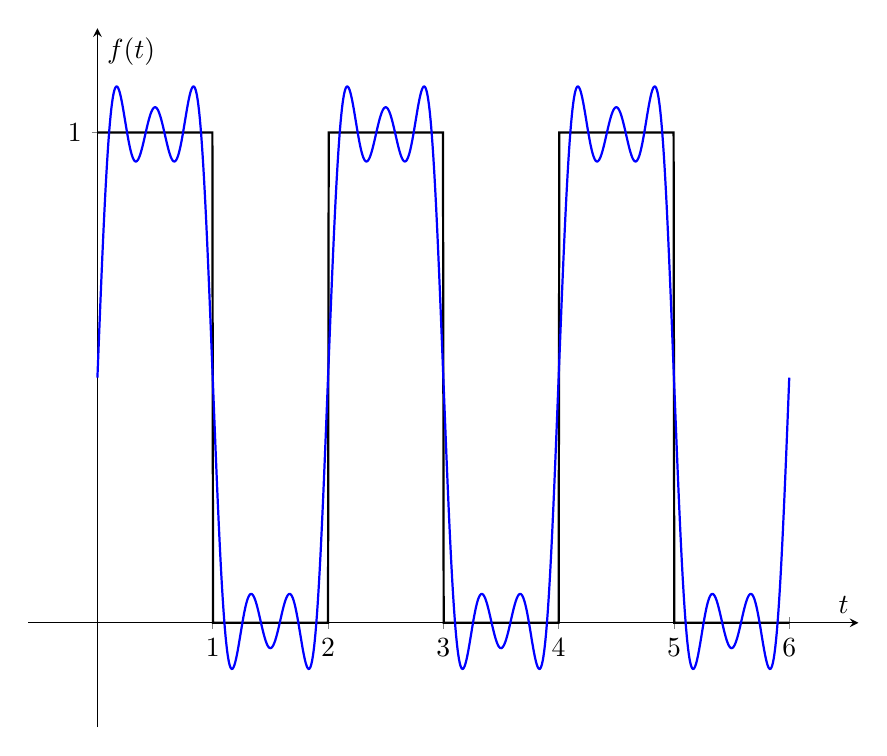
\begin{tikzpicture}
	\begin{axis}[
		axis lines = middle,
		xlabel = {$t$},
		ylabel = {$f(t)$},		
		domain=0:6,
		samples=1000,
		xtick={0,1,2,3,4,5,6},
		ytick={0,1},
		enlargelimits,
		width=\textwidth
		]
		\addplot[thick] {mod(floor(x),2) == 0 ? 1 : 0};
		\addplot[blue, thick] {(1/2) + 
			(2/pi)*sin(pi * deg(x)) + 
			(2/(3*pi))*sin(pi *3*deg(x)) +
			(2/(5*pi))*sin(pi *5*deg(x))};
	\end{axis}
\end{tikzpicture}

$a_0$ ist bei 


\subsection{Fouriertransformation\label{fourier:subsection:fouriertransformation}}


%
% teil1.tex -- Beispiel-File für das Paper
%
% (c) 2020 Prof Dr Andreas Müller, Hochschule Rapperswil
%
% !TEX root = ../../buch.tex
% !TEX encoding = UTF-8
%
\section{Metrik und Hodge-Theorie 
\label{maxwell:section:teil1}}
\kopfrechts{Metrik und Hodge-Theorie}

\subsection{Minkowski Metrik}
In der speziellen Relativitätstheorie (SRT) wird die Minkowski-Metrik verwendet.
\index{spezielle Relativitätstheorie}%
\index{Relativitätstheorie, spezielle}%
\index{Minkowski-Metrik}%
Da es in der SRT keine Krümmung und Gravitation gibt, sind alle Elemente ausserhalb der Diagonale des metrischen Tensors null und somit ist die Raum-Zeit flach.
Zwei Signaturen sind üblich.
Einerseits gibt es die $({-}{+}{+}{+})$-Signatur, bei welcher die Zeitkomponente negativ und die Raumkomponenten positiv gezählt werden.
Andererseits gibt es die $({+}{-}{-}{-})$-Signatur, bei welcher die Zeitkomponente positiv und die Raumkomponenten negativ gezählt werden.
Beide Signaturen sind gleichwertig, solange man sich auf eine Metrik festlegt und diese konsequent beibehält.
Im Folgenden werden wir uns an die $({-}{+}{+}{+})$-Signatur halten.
Daher definieren wir den metrischen Tensor als
\begin{equation}
	g^{ik} = \begin{pmatrix}
		-1 & 0 & 0 & 0 \\ 0 & 1 & 0 & 0 \\ 0 & 0 & 1 & 0 \\ 0 & 0 & 0 & 1 
	\end{pmatrix}.
	\label{maxwell:section:teil1:metrik}
\end{equation}
Der Ausdruck für ein Linienelement in dieser Metrik ist definiert als
\begin{equation*}
	dl^2 = -(dx^0)^2 +(dx^1)^2+(dx^2)^2+(dx^3)^2.
\end{equation*}
Damit wir Raum und Zeit in dieser Metrik gleichartig behandeln können, wählen wir beim Übergang in physikalische Einheiten 
\begin{equation}
	\label{maxwell:koordinaten}
	x^0 = ct,\quad x^1 = x,\quad x^2 = y, \quad x^3 = z .
\end{equation}
Dabei entspricht $c$ der Lichtgeschwindigkeit und ein Linienelement ist somit definiert als
\begin{equation*}
	dl^2 = -c^2dt^2 +dx^2+dy^2+dz^2.
\end{equation*}
Eine Konsequenz dieser Signatur ist, dass zeitartige Abstände $dl^2 < 0$ und raumartige Abstände $dl^2 > 0$ sind.

\subsection{Hodge-Duale der Basis-$k$-Formen}
Für den Teil der inhomogenen Maxwell-Gleichungen benötigen wir die Hodge-Duale von 1-Formen, 2-Formen und 3-Formen im vierdimensionalen Minkowski-Raum.
Um dabei die korrekten Vorzeichen zu erhalten, muss die Hodge-Dualität mit Hilfe des metrischen Tensors $g^{ik}$  der Minkowski-Metrik verwendet werden.

Wir verwenden die Definition des Hodge-Operators
\begin{equation*}
	\alpha \wedge \ast \beta = \langle \alpha, \beta \rangle \operatorname{vol}(M),
\end{equation*}
wobei $\langle \cdot , \cdot \rangle$ das durch die Metrik $g^{ik}$ induzierte Skalarprodukt ist.
Im Folgenden führen wir alle Berechnungen der Hodge-Duale von 1-, 2- und 3-Formen durch.
Wir verwenden $g^{ik}$ gemäss \eqref{maxwell:section:teil1:metrik} und $\operatorname{vol}(M) = dx^0 \wedge dx^1 \wedge dx^2 \wedge dx^3$.
\begin{definition}
\label{maxwell:hodge:kurzschreibweise}
Um die Notation kompakter und übersichtlicher zu gestalten, führen wir die Schreibweise
\begin{align*}
	dx^{i\!j} &:= dx^i \wedge dx^j, 
	%\label{maxwell:hodge:zwei}
	\\
	dx^{i\!jk} &:= dx^i \wedge dx^j \wedge dx^k, 
	%\label{maxwell:hodge:drei}
	\\
	dx^{i\!jkl} & := dx^i \wedge dx^j \wedge dx^k \wedge dx^l
	\notag
\end{align*}
für Wedge-Produkte von Basisformen ein.
\end{definition}
Mit dieser Vorbereitung können wir nun die konkreten Hodge-Duale der Basisformen berechnen.
\subsubsection{Hodge-Duale von 1-Formen}
\begin{align*}
	\ast dx^0 
	&= s \, dx^{123} \\
	dx^0 \wedge \ast dx^0 
	&= dx^0 \wedge s \, dx^{123} = s \, dx^{0123} \\
	&= \langle dx^0, dx^0 \rangle \operatorname{vol}(M) = g^{00} \, dx^{0123} = -dx^{0123} \\
	\Rightarrow s &= -1 \Rightarrow \boxed{\ast dx^0 = - dx^{123}}
	\\[1em]
	\ast dx^1 
	&= s \, dx^{023} \\
	dx^1 \wedge \ast dx^1 
	&= dx^1 \wedge s \, dx^{023} = -s \, dx^{0123} \\
	&= \langle dx^1, dx^1 \rangle \operatorname{vol}(M) = g^{11} \, dx^{0123} = dx^{0123} \\
	\Rightarrow s &= -1 \Rightarrow \boxed{\ast dx^1 = - dx^{023}}
	\\[1em]
	\ast dx^2 
	&= s \, dx^{013} \\
	dx^2 \wedge \ast dx^2 
	&= dx^2 \wedge s \, dx^{013} = s \, dx^{0123} \\
	&= \langle dx^2, dx^2 \rangle \operatorname{vol}(M) = g^{22} \, dx^{0123} = dx^{0123} \\
	\Rightarrow s &= +1 \Rightarrow \boxed{\ast dx^2 = dx^{013}}
	\\[1em]
	\ast dx^3 
	&= s \, dx^{012} \\
	dx^3 \wedge \ast dx^3 
	&= dx^3 \wedge s \, dx^{012} = -s \, dx^{0123} \\
	&= \langle dx^3, dx^3 \rangle \operatorname{vol}(M) = g^{33} \, dx^{0123} = dx^{0123} \\
	\Rightarrow s &= -1 \Rightarrow \boxed{\ast dx^3 = - dx^{012}}
\end{align*}

\subsubsection{Hodge-Duale von 2-Formen}
\begin{align*}
	\ast dx^{01} &= s \, dx^{23} \\
	dx^{01} \wedge \ast dx^{01} &= s \, dx^{0123} \\
	&= \langle dx^{01}, dx^{01} \rangle \, \operatorname{vol}(M) 
	= g^{00} g^{11} \operatorname{vol}(M) = -dx^{0123} \\
	\Rightarrow s &= -1 \Rightarrow \boxed{\ast dx^{01} = - dx^{23}}
	\\[1em]
	\ast dx^{12} &= s \, dx^{03} \\
	dx^{12} \wedge \ast dx^{12} &= s \, dx^{0123} \\
	&= \langle dx^{12}, dx^{12} \rangle \, \operatorname{vol}(M) 
	= g^{11} g^{22} \operatorname{vol}(M) = dx^{0123} \\
	\Rightarrow s &= +1 \Rightarrow \boxed{\ast dx^{12} = dx^{03}}
	\\[1em]
	\ast dx^{23} &= s \, dx^{01} \\
	dx^{23} \wedge \ast dx^{23} &= s \, dx^{0123} \\
	&= \langle dx^{23}, dx^{23} \rangle \, \operatorname{vol}(M) 
	= g^{22} g^{33} \operatorname{vol}(M) = dx^{0123} \\
	\Rightarrow s &= +1 \Rightarrow \boxed{\ast dx^{23} = dx^{01}}
	\\[1em]
	\ast dx^{02} &= s \, dx^{13} \\
	dx^{02} \wedge \ast dx^{02} &= -s \, dx^{0123} \\
	&= \langle dx^{02}, dx^{02} \rangle \, \operatorname{vol}(M) 
	= g^{00} g^{22} \operatorname{vol}(M) = -dx^{0123} \\
	\Rightarrow s &= +1 \Rightarrow \boxed{\ast dx^{02} = dx^{13}}
	\\[1em]
	\ast dx^{03} &= s \, dx^{12} \\
	dx^{03} \wedge \ast dx^{03} &= s \, dx^{0123} \\
	&= \langle dx^{03}, dx^{03} \rangle \, \operatorname{vol}(M) 
	= g^{00} g^{33} \operatorname{vol}(M) = -dx^{0123} \\
	\Rightarrow s &= -1 \Rightarrow \boxed{\ast dx^{03} = - dx^{12}}
	\\[1em]
	\ast dx^{13} &= s \, dx^{02} \\
	dx^{13} \wedge \ast dx^{13} &= -s \, dx^{0123} \\
	&= \langle dx^{13}, dx^{13} \rangle \, \operatorname{vol}(M) 
	= g^{11} g^{33} \operatorname{vol}(M) = dx^{0123} \\
	\Rightarrow s &= -1 \Rightarrow \boxed{\ast dx^{13} = - dx^{02}}
\end{align*}

\subsubsection{Hodge-Duale von 3-Formen}
\begin{align*}
	\ast dx^{012} &= s \, dx^3 \\
	dx^{012} \wedge \ast dx^{012} &= s \, dx^{0123} \\
	&= \langle dx^{012}, dx^{012} \rangle \, \operatorname{vol}(M) 
	= g^{00} g^{11} g^{22} \operatorname{vol}(M) = -dx^{0123} \\
	\Rightarrow s &= -1 \Rightarrow \boxed{\ast dx^{012} = - dx^3}
	\\[1em]
	\ast dx^{013} &= s \, dx^2 \\
	dx^{013} \wedge \ast dx^{013} &= -s \, dx^{0123} \\
	&= \langle dx^{013}, dx^{013} \rangle \, \operatorname{vol}(M) 
	= g^{00} g^{11} g^{33} \operatorname{vol}(M) = -dx^{0123} \\
	\Rightarrow s &= 1 \Rightarrow \boxed{\ast dx^{013} = dx^2}
	\\[1em]
	\ast dx^{023} &= s \, dx^1 \\
	dx^{023} \wedge \ast dx^{023} &= s \, dx^{0123} \\
	&= \langle dx^{023}, dx^{023} \rangle \, \operatorname{vol}(M) 
	= g^{00} g^{22} g^{33} \operatorname{vol}(M) = -dx^{0123} \\
	\Rightarrow s &= -1 \Rightarrow \boxed{\ast dx^{023} = - dx^1}
	\\[1em]
	\ast dx^{123} &= s \, dx^0 \\
	dx^{123} \wedge \ast dx^{123} &= -s \, dx^{0123} \\
	&= \langle dx^{123}, dx^{123} \rangle \, \operatorname{vol}(M)
	= g^{11} g^{22} g^{33} \operatorname{vol}(M) = dx^{0123} \\
	\Rightarrow s &= -1 \Rightarrow \boxed{\ast dx^{123} = - dx^0}
\end{align*}
In der Tabelle \ref{maxwell:section:teil1:Hodge-Tabelle} sind alle berechneten Hodge-Duale noch einmal zusammengefasst.
\begin{table}
	\centering
	%\caption{Hodge-Duale}
	%\label{maxwell:section:teil1:Hodge-Tabelle}
	\begin{tabularx}{\textwidth}{ 
			| >{\centering\arraybackslash}X 
			| >{\centering\arraybackslash}X 
			| >{\centering\arraybackslash}X | }
		\hline
		\textbf{1-Form} & \textbf{2-Form} & \textbf{3-Form} \\
		\hline
		\( \rule{0pt}{1.5em} {\ast} dx^0 = -dx^1 \wedge dx^2 \wedge dx^3 \) \newline
	\( {\ast} dx^1 = -dx^0 \wedge dx^2 \wedge dx^3 \) \newline
	\( {\ast} dx^2 = \phantom{-} dx^0 \wedge dx^1 \wedge dx^3 \) \newline
	\( {\ast} dx^3 = -dx^0 \wedge dx^1 \wedge dx^2 \, \) 
	&
	\( \rule{0pt}{1.5em} {\ast} (dx^0 \wedge dx^1) = -dx^2 \wedge dx^3 \) \newline
	\( {\ast} (dx^1 \wedge dx^2) = \phantom{-} dx^0 \wedge dx^3 \) \newline
	\( {\ast} (dx^2 \wedge dx^3) = \phantom{-} dx^0 \wedge dx^1 \) \newline
	\( {\ast} (dx^0 \wedge dx^2) = \phantom{-} dx^1 \wedge dx^3 \) \newline
	\( {\ast} (dx^0 \wedge dx^3) = -dx^1 \wedge dx^2 \) \newline
	\( {\ast} (dx^1 \wedge dx^3) = -dx^0 \wedge dx^2 \)
	&
	\( \rule{0pt}{1.5em} {\ast} (dx^0 \wedge dx^1 \wedge dx^2) = -dx^3 \) \newline
	\( {\ast} (dx^0 \wedge dx^1 \wedge dx^3) = \phantom{-} dx^2 \) \newline
	\( {\ast} (dx^0 \wedge dx^2 \wedge dx^3) = -dx^1 \) \newline
	\( {\ast} (dx^1 \wedge dx^2 \wedge dx^3) = -dx^0 \)
		\\
		\hline
	\end{tabularx}
	\caption{Tabelle aller Hodge-Duale von 1-, 2-, und 3-Formen mit $({-}{+}{+}{+})$-Signatur}
	\label{maxwell:section:teil1:Hodge-Tabelle}
\end{table}








\section{Homogene Maxwellgleichungen}
Die homogenen Maxwellgleichungen bekommen wir durch die äussere Ableitung des Feldstärketensors, den wir in (Abschnitt vom Herr widmer, ref) durch $F = dA$ erhalten haben
\[
F_{\mu\nu}
= 
\begin{pmatrix}
	0 & -E_1 & -E_2 & -E_3 \\
	E_1 &  0 &  B_3 & -B_2 \\
	E_2 & -B_3 &  0 &  B_1 \\
	E_3 &  B_2 & -B_1 &  0 \\
\end{pmatrix}.
\]
Wir wissen, aus (ref Buch dd=0), das
\[
ddA = dF = 0
\]
gelten muss.
Für die Berechnung der äusseren Ableitung muss der Tensor zuerst als Differentialform geschrieben werden.
Es resultiert die Zweiform
\[
F
= \frac{1}{2} F_{\mu\nu} \, dx^\mu \wedge dx^\nu,
\]
man beachte dabei die einsteinsche Summationskonvention(ref Buch?).
Da der Feldstärketensor antisymmetrisch $F_{\mu\nu} = -F_{\nu\mu}$ ist, benötigt man den Faktor $\frac{1}{2}$ um die doppelte Zählung der Komponenten zu vermeiden:
\begin{align*}
	F
	= 
	&+ \frac{1}{2} F_{\mu\nu} \, dx^\mu \wedge dx^\nu
	\\
	=
	&+ \frac{1}{2} F_{00} \, dx^0 \wedge dx^0 + \frac{1}{2} F_{01} \, dx^0 \wedge dx^1 + \frac{1}{2} F_{02} \, dx^0 \wedge dx^2 + \frac{1}{2} F_{03} \, dx^0 \wedge dx^3
	\\
	&+ \frac{1}{2} F_{10} \, dx^1 \wedge dx^0 + \frac{1}{2} F_{11} \, dx^1 \wedge dx^1 + \frac{1}{2} F_{12} \, dx^1 \wedge dx^2 + \frac{1}{2} F_{13} \, dx^1 \wedge dx^3
	\\
	&+ \frac{1}{2} F_{20} \, dx^2 \wedge dx^0 + \frac{1}{2} F_{21} \, dx^2 \wedge dx^1 + \frac{1}{2} F_{22} \, dx^2 \wedge dx^2 + \frac{1}{2} F_{23} \, dx^2 \wedge dx^3
	\\
	&+ \frac{1}{2} F_{30} \, dx^3 \wedge dx^0 + \frac{1}{2} F_{31} \, dx^3 \wedge dx^1 + \frac{1}{2} F_{32} \, dx^3 \wedge dx^2 + \frac{1}{2} F_{33} \, dx^3 \wedge dx^3
\end{align*} 
Da gilt $dx^n \wedge dx^n = 0$ und $dx^n \wedge dx^{n+1} = - dx^{n+1} \wedge dx^n$, folgt nach aufsteigenden Indizes sortiert
\begin{align*}
	F
	=
	&+ \frac{1}{2} F_{01} \, dx^0 \wedge dx^1 + \frac{1}{2} F_{02} \, dx^0 \wedge dx^2 + \frac{1}{2} F_{03} \, dx^0 \wedge dx^3
	\\
	&- \frac{1}{2} F_{10} \, dx^0 \wedge dx^1 + \frac{1}{2} F_{12} \, dx^1 \wedge dx^2 + \frac{1}{2} F_{13} \, dx^1 \wedge dx^3
	\\
	&- \frac{1}{2} F_{20} \, dx^0 \wedge dx^2 - \frac{1}{2} F_{21} \, dx^1 \wedge dx^2 + \frac{1}{2} F_{23} \, dx^2 \wedge dx^3
	\\
	&- \frac{1}{2} F_{30} \, dx^0 \wedge dx^3 - \frac{1}{2} F_{31} \, dx^1 \wedge dx^3 - \frac{1}{2} F_{32} \, dx^2 \wedge dx^3
\end{align*}
und wegen $F_{\mu\nu} = -F_{\nu\mu}$
\begin{align*}
	F
	=
	&+ \frac{1}{2} F_{01} \, dx^0 \wedge dx^1 + \frac{1}{2} F_{02} \, dx^0 \wedge dx^2 + \frac{1}{2} F_{03} \, dx^0 \wedge dx^3
	\\
	&+ \frac{1}{2} F_{01} \, dx^0 \wedge dx^1 + \frac{1}{2} F_{12} \, dx^1 \wedge dx^2 + \frac{1}{2} F_{13} \, dx^1 \wedge dx^3
	\\
	&+ \frac{1}{2} F_{02} \, dx^0 \wedge dx^2 + \frac{1}{2} F_{12} \, dx^1 \wedge dx^2 + \frac{1}{2} F_{23} \, dx^2 \wedge dx^3
	\\
	&+ \frac{1}{2} F_{03} \, dx^0 \wedge dx^3 + \frac{1}{2} F_{13} \, dx^1 \wedge dx^3 + \frac{1}{2} F_{23} \, dx^2 \wedge dx^3
	\\
	\\
	=
	&+ \frac{1}{2} F_{01} \, dx^0 \wedge dx^1 + \frac{1}{2} F_{02} \, dx^0 \wedge dx^2 + \frac{1}{2} F_{03} \, dx^0 \wedge dx^3
	\\
	&+ \frac{1}{2} F_{12} \, dx^1 \wedge dx^2 + \frac{1}{2} F_{13} \, dx^1 \wedge dx^3 + \frac{1}{2} F_{23} \, dx^2 \wedge dx^3 \, .
\end{align*}
Für besseres Verständnis setzen wir nun konkret die Komponenten von $F_{\mu\nu}$ ein und erhalten
 \begin{align*}
 	F
 	=
 	&- \frac{1}{2} E_1 \, dx^0 \wedge dx^1 - \frac{1}{2} E_2 \, dx^0 \wedge dx^2 - \frac{1}{2} E_3 \, dx^0 \wedge dx^3
 	\\
 	&+ \frac{1}{2} B_3 \, dx^1 \wedge dx^2 - \frac{1}{2} B_2 \, dx^1 \wedge dx^3 + \frac{1}{2} B_1 \, dx^2 \wedge dx^3 \, ,
 \end{align*}
was schön den Komponenten oberhalb der Diagonalen von $F_{\mu\nu}$ entspricht.
Nun wenden wir die äussere Ableitung auf die Zweiform F an
 \begin{align*}
 	dF =
 	&\cancel{\, - \, \frac{\d E_1}{\d x^0} \, dx^0 \wedge dx^0 \wedge dx^1} \cancel{\, - \, \frac{\d E_1}{\d x^1} \, dx^1 \wedge dx^0 \wedge dx^1}
 	 - \frac{\d E_1}{\d x^2} \, dx^2 \wedge dx^0 \wedge dx^1 - \frac{\d E_1}{\d x^3} \, dx^3 \wedge dx^0 \wedge dx^1
 	\\
 	&\cancel{\, - \, \frac{\d E_2}{\d x^0} \, dx^0 \wedge dx^0 \wedge dx^2} - \frac{\d E_2}{\d x^1} \, dx^1 \wedge dx^0 \wedge dx^2
 	 \cancel{\, - \, \frac{\d E_2}{\d x^2} \, dx^2 \wedge dx^0 \wedge dx^2} - \frac{\d E_2}{\d x^3} \, dx^3 \wedge dx^0 \wedge dx^2
 	\\
 	&\cancel{\, - \, \frac{\d E_3}{\d x^0} \, dx^0 \wedge dx^0 \wedge dx^3} - \frac{\d E_3}{\d x^1} \, dx^1 \wedge dx^0 \wedge dx^3
 	 - \frac{\d E_3}{\d x^2} \, dx^2 \wedge dx^0 \wedge dx^3 \cancel{\, - \, \frac{\d E_3}{\d x^3} \, dx^3 \wedge dx^0 \wedge dx^3}
 	\\
 	&+ \frac{\d B_3}{\d x^0} \, dx^0 \wedge dx^1 \wedge dx^2 \cancel{\, + \, \frac{\d B_3}{\d x^1} \, dx^1 \wedge dx^1 \wedge dx^2}
 	 \cancel{\, + \, \frac{\d B_3}{\d x^2} \, dx^2 \wedge dx^1 \wedge dx^2} + \frac{\d B_3}{\d x^3} \, dx^3 \wedge dx^1 \wedge dx^2
 	\\
 	&- \frac{\d B_2}{\d x^0} \, dx^0 \wedge dx^1 \wedge dx^3 \cancel{\, - \, \frac{\d B_2}{\d x^1} \, dx^1 \wedge dx^1 \wedge dx^3}
 	 - \frac{\d B_2}{\d x^2} \, dx^2 \wedge dx^1 \wedge dx^3 \cancel{\, - \, \frac{\d B_2}{\d x^3} \, dx^3 \wedge dx^1 \wedge dx^3}
 	\\
 	&+ \frac{\d B_1}{\d x^0} \, dx^0 \wedge dx^2 \wedge dx^3 + \frac{\d B_1}{\d x^1} \, dx^1 \wedge dx^2 \wedge dx^3
 	 \cancel{\, + \, \frac{\d B_1}{\d x^2} \, dx^2 \wedge dx^2 \wedge dx^3} \cancel{\, + \, \frac{\d B_1}{\d x^3} \, dx^3 \wedge dx^2 \wedge dx^3}
 	\\
 	\\
 	=
 	&- \frac{\d E_1}{\d x^2} \, dx^2 \wedge dx^0 \wedge dx^1 - \frac{\d E_1}{\d x^3} \, dx^3 \wedge dx^0 \wedge dx^1
 	 - \frac{\d E_2}{\d x^1} \, dx^1 \wedge dx^0 \wedge dx^2 - \frac{\d E_2}{\d x^3} \, dx^3 \wedge dx^0 \wedge dx^2
 	\\
 	&- \frac{\d E_3}{\d x^1} \, dx^1 \wedge dx^0 \wedge dx^3 - \frac{\d E_3}{\d x^2} \, dx^2 \wedge dx^0 \wedge dx^3
 	 + \frac{\d B_3}{\d x^0} \, dx^0 \wedge dx^1 \wedge dx^2 + \frac{\d B_3}{\d x^3} \, dx^3 \wedge dx^1 \wedge dx^2
 	\\
 	&- \frac{\d B_2}{\d x^0} \, dx^0 \wedge dx^1 \wedge dx^3 - \frac{\d B_2}{\d x^2} \, dx^2 \wedge dx^1 \wedge dx^3
 	 + \frac{\d B_1}{\d x^0} \, dx^0 \wedge dx^2 \wedge dx^3 + \frac{\d B_1}{\d x^1} \, dx^1 \wedge dx^2 \wedge dx^3 \, , 
 \end{align*}
sortieren nach aufsteigenden Indizes
 \begin{align*}
	dF =
	&- \frac{\d E_1}{\d x^2} \, dx^0 \wedge dx^1 \wedge dx^2 - \frac{\d E_1}{\d x^3} \, dx^0 \wedge dx^1 \wedge dx^3
	 + \frac{\d E_2}{\d x^1} \, dx^0 \wedge dx^1 \wedge dx^2 - \frac{\d E_2}{\d x^3} \, dx^0 \wedge dx^2 \wedge dx^3
	\\
	&+ \frac{\d E_3}{\d x^1} \, dx^0 \wedge dx^1 \wedge dx^3 + \frac{\d E_3}{\d x^2} \, dx^0 \wedge dx^2 \wedge dx^3
	 + \frac{\d B_3}{\d x^0} \, dx^0 \wedge dx^1 \wedge dx^2 + \frac{\d B_3}{\d x^3} \, dx^1 \wedge dx^2 \wedge dx^3
	\\
	&- \frac{\d B_2}{\d x^0} \, dx^0 \wedge dx^1 \wedge dx^3 + \frac{\d B_2}{\d x^2} \, dx^1 \wedge dx^2 \wedge dx^3
	 + \frac{\d B_1}{\d x^0} \, dx^0 \wedge dx^2 \wedge dx^3 + \frac{\d B_1}{\d x^1} \, dx^1 \wedge dx^2 \wedge dx^3
\end{align*}
und fassen anschliessend alles zusammen
\begin{align*}
	dF =
	&\left( - \frac{\d E_1}{\d x^2} + \frac{\d E_2}{\d x^1} + \frac{\d B_3}{\d x^0} \right) dx^0 \wedge dx^1 \wedge dx^2
	\\
	+&\left( - \frac{\d E_1}{\d x^3} + \frac{\d E_3}{\d x^1} - \frac{\d B_2}{\d x^0} \right) dx^0 \wedge dx^1 \wedge dx^3
	\\
	+&\left( - \frac{\d E_2}{\d x^3} + \frac{\d E_3}{\d x^2} + \frac{\d B_1}{\d x^0} \right) dx^0 \wedge dx^2 \wedge dx^3
	\\
	+&\left( + \frac{\d B_3}{\d x^3} + \frac{\d B_2}{\d x^2} + \frac{\d B_1}{\d x^1} \right) dx^1 \wedge dx^2 \wedge dx^3 \, .
\end{align*}
\textbf{Aussage Unsicher!:} Da die Vorzeichen der partiellen Ableitung nicht passen, ändern wir dort die Reihenfolge der Wedgeprodukte
\begin{align*}
	dF =
	&\left( - \frac{\d E_1}{\d x^2} + \frac{\d E_2}{\d x^1} + \frac{\d B_3}{\d x^0} \right) dx^0 \wedge dx^1 \wedge dx^2
	\\
	+&\left( + \frac{\d E_1}{\d x^3} - \frac{\d E_3}{\d x^1} + \frac{\d B_2}{\d x^0} \right) dx^0 \wedge dx^3 \wedge dx^1
	\\
	+&\left( - \frac{\d E_2}{\d x^3} + \frac{\d E_3}{\d x^2} + \frac{\d B_1}{\d x^0} \right) dx^0 \wedge dx^2 \wedge dx^3
	\\
	+&\left( + \frac{\d B_3}{\d x^3} + \frac{\d B_2}{\d x^2} + \frac{\d B_1}{\d x^1} \right) dx^1 \wedge dx^2 \wedge dx^3 \, .
\end{align*}
und erkennen nun, wenn $dx^0 = dt, dx^1 = dx, dx^2 = dy, dx^3 = dz$:
\begin{align*}
	dF =
	&\Bigg( \underbrace{ - \frac{\d E_x}{\d y} + \frac{\d E_y}{\d x}}_{(\nabla \times E)_z} + \frac{\d B_z}{\d t} \Bigg) dt \wedge dx \wedge dy
	\\
	+&\Bigg( \underbrace{ + \frac{\d E_x}{\d z} - \frac{\d E_z}{\d x}}_{(\nabla \times E)_y} + \frac{\d B_y}{\d t} \Bigg) dt \wedge dz \wedge dx
	\\
	+&\Bigg( \underbrace{ - \frac{\d E_y}{\d z} + \frac{\d E_z}{\d y}}_{(\nabla \times E)_x} + \frac{\d B_x}{\d t} \Bigg) dt \wedge dy \wedge dz
	\\
	+&\Bigg( \underbrace{ + \frac{\d B_z}{\d z} + \frac{\d B_y}{\d y} + \frac{\d B_x}{\d x}}_{\nabla \cdot \vec{B}} \Bigg) dx \wedge dy \wedge dz \, .
\end{align*}
Das sind genau die homogenen Maxwellgleichungen
\[
\nabla \times \vec{E} + \frac{\d \vec{B}}{\d t} = 0
\]
und
\[
\nabla \cdot \vec{B} = 0 \, .
\]
%
% InhomogeneMaxwellgleichungen.tex -- Beispiel-File für das Paper
%
% (c) 2020 Prof Dr Andreas Müller, Hochschule Rapperswil
%
% !TEX root = ../../buch.tex
% !TEX encoding = UTF-8
%
\section{Inhomogene Maxwell-Gleichungen
	\label{maxwell:section:InhomogeneMaxwellgleichungen}}
\kopfrechts{Inhomogene Maxwellgleichungen}
Den Faraday-Tensor haben wir definiert als
\begin{equation*}
	F_{\mu \nu} = \begin{pmatrix}
		0 & -E_1/c & -E_2/c & -E_3/c \\ E_1/c & 0 & B_3 & -B_2 \\ E_2/c & -B_3 & 0 & B_1 \\ E_3/c & B_2 & -B_1 & 0 
	\end{pmatrix}.
\end{equation*}
Wir haben dabei festgestellt, dass die äussere Ableitung von $F$ verschwindet, da $F$ eine geschlossene 2-Form ist. Dadurch haben wir die homogenen Maxwell-Gleichungen erhalten. 
%Um nun die inhomogenen Maxwell-Gleichungen bestimmen zu können, müssen wir den Hodge-Operator auf $F$ anwenden.

Um nun die inhomogenen Maxwell-Gleichungen bestimmen zu können, benötigen wir eine Art Verallgemeinerung der Divergenz, die das Quellenverhalten des Faraday-Tensors misst. Hierfür eignet sich das Kodifferential
\begin{equation*}
	\delta = \ast d {\ast}.
\end{equation*}
%Diese Operation erlaubt es, quellenartige Beiträge geometrisch zu erfassen.
Aus den klassischen inhomogenen Maxwell-Gleichungen
\begin{align}
	\nabla \cdot \vec{E} &= \frac{\rho}{\varepsilon_0}
	\label{maxwell:section:inhomogeneMaxwellgleichungen:gaussE},\\
	\nabla \times \vec{B} - \varepsilon_0 \mu_0 \frac{\partial \vec{E}}{\partial t}&= \mu_0 \vec{J}
	\label{maxwell:section:inhomogeneMaxwellgleichungen:ampereMaxwell}
\end{align}
erkennen wir, welche Operationen mit $\vec{E}$ und $\vec{B}$ gemacht werden müssen.
Da im Faraday-Tensor die elektrische Feldstärke $\vec{E}$ und die magnetische Flussdichte $\vec{B}$ enthalten sind, wenden wir das Kodifferential auf $F$ an und untersuchen, ob die obigen Operationen in der Sprache der Differentialformen herauskommen.

Damit wir wissen, welche geometrische Form die Operation 
\begin{equation*}
	\delta F = \ast d{\ast} F
\end{equation*}
haben wird, überlegen wir uns, was der Hodge-Operator und die äussere Ableitung mit dem Grad machen.

Der Hodge-Operator bildet eine $k$-Form auf eine $(n-k)$-Form ab.
Da wir uns im vierdimensionalen Minkowsky-Raum befinden, wird durch Anwendung des Hodge-Operators auf die 2-Form $F$ wieder eine 2-Form.
Die Anwendung der äusseren Ableitung erhöht den Grad um eins und ergibt somit eine 3-Form.
Durch erneutes Anwenden des Hodge-Operators entsteht schliesslich eine 1-Form.

Aus den Gleichungen \eqref{maxwell:section:inhomogeneMaxwellgleichungen:gaussE} und \eqref{maxwell:section:inhomogeneMaxwellgleichungen:ampereMaxwell} sehen wir, dass auf der rechten Seite Terme in Form von Ladungs- und Stromdichten auftreten.
Es liegt nahe, auch $\rho$ und $\vec{J}$ zu einem einzigen geometrischen Objekt zusammenzufassen, da beide Quellenterme darstellen.
Das Ziel dabei ist, die beiden inhomogenen Maxwell-Gleichungen in einer einzigen Gleichung zusammenzufassen.

Folglich muss das geometrische Objekt, welches die Ladungs- und Stromdichte enthält, eine 1-Form sein.
Diese werden wir zukünftig Viererstromdichte $J$ nennen.
Sobald wir das $\ast d {\ast} F$ berechnet haben, definieren wir $J$ so, dass die Gleichung aufgeht.

\subsection{Berechnung des Kodifferentials von $F$}

Wir erinnern uns, dass $F$ ausgeschrieben mit Wedge-Produkten definiert ist als
\begin{align*}
	F = 
	- &\frac{E_{1}}{c} \, dx^0 \wedge dx^1 - \frac{E_{2}}{c} \, dx^0 \wedge dx^2 - \frac{E_{3}}{c} \, dx^0 \wedge dx^3 \\
	+ & \, B_3 \, \, dx^1 \wedge dx^2 - B_2 \, \, dx^1 \wedge dx^3 + \, B_1 \, \, dx^2 \wedge dx^3.
\end{align*}

\subsubsection{Berechnung von $\ast F$}
Zuerst wenden wir den Hodge-Operator auf $F$ an und erhalten
\begin{align*}
	\ast F =
	& - \frac{E_{1}}{c} \, {\ast}(dx^0 \wedge dx^1) - \frac{E_{2}}{c} \, {\ast}(dx^0 \wedge dx^2) - \frac{E_{3}}{c} \, {\ast}(dx^0 \wedge dx^3) \\
	& + \, B_3 \, \, {\ast}(dx^1 \wedge dx^2) - \, B_2 \, \, {\ast}(dx^1 \wedge dx^3) + B_1 \, {\ast}(dx^2 \wedge dx^3).
\end{align*}
Die Hodge-Duale können aus der Tabelle \ref{maxwell:section:teil1:Hodge-Tabelle} entnommen werden und wir erhalten
\begin{align*}
	\ast F =
	& \, \frac{E_{1}}{c} \, dx^2 \wedge dx^3 - \frac{E_{2}}{c} \, dx^1 \wedge dx^3 + \frac{E_{3}}{c} \, dx^1 \wedge dx^2 \\
	 + & \, B_3 \, \, dx^0 \wedge dx^3 + \, B_2 \, \, dx^0 \wedge dx^2 + \, B_1 \, \, dx^0 \wedge dx^1.
\end{align*}
Die erhaltene 2-Form kann nun wieder als Matrix
\begin{equation}
	\ast F = \begin{pmatrix}
		0 & B_1 & B_2 & B_3 \\ -B_1 & 0 & E_3/c & -E_2/c \\ -B_2 & -E_3/c & 0 & E_1/c \\ -B_3 & E_2/c & -E_1/c & 0 
	\end{pmatrix}
	%	\label{maxwell:section:teil1:metrik}
\end{equation}
geschrieben werden.
Wir sehen, dass durch den Hodge-Operator die $E$ und $B$ ihre Plätze tauschen.
\subsubsection{Berechnung von $d {\ast} F$}
Nun wenden wir die äussere Ableitung an und erhalten
\begin{align*}
	d{\ast} F
	= &\phantom{+} d \, \Bigg(
	\frac{E_{1}}{c} \, dx^2 \wedge dx^3
	- \frac{E_{2}}{c} \, dx^1 \wedge dx^3
	+ \frac{E_{3}}{c} \, dx^1 \wedge dx^2 
	\\
	&+ B_3 \, dx^0 \wedge dx^3
	+ B_2 \, dx^0 \wedge dx^2
	+ B_1 \, dx^0 \wedge dx^1
	\Bigg) \\[1ex]
	= \phantom{+} &\frac{1}{c} \frac{\partial E_1}{\partial x^0} \, dx^0 \wedge dx^2 \wedge dx^3
	+ \frac{1}{c} \frac{\partial E_1}{\partial x^1} \, dx^1 \wedge dx^2 \wedge dx^3
	- \frac{1}{c} \frac{\partial E_2}{\partial x^0} \, dx^0 \wedge dx^1 \wedge dx^3 
	\\
	- &\frac{1}{c} \frac{\partial E_2}{\partial x^2} \, dx^2 \wedge dx^1 \wedge dx^3
	+ \frac{1}{c} \frac{\partial E_3}{\partial x^0} \, dx^0 \wedge dx^1 \wedge dx^2
	+ \frac{1}{c} \frac{\partial E_3}{\partial x^3} \, dx^3 \wedge dx^1 \wedge dx^2 
	\\
	+&\phantom{\frac{1}{c}} \frac{\partial B_3}{\partial x^1} \, dx^1 \wedge dx^0 \wedge dx^3
	+ \phantom{\frac{1}{c}} \frac{\partial B_3}{\partial x^2} \, dx^2 \wedge dx^0 \wedge dx^3
	+ \phantom{\frac{1}{c}} \frac{\partial B_2}{\partial x^1} \, dx^1 \wedge dx^0 \wedge dx^2 \\
	+&\phantom{\frac{1}{c}} \frac{\partial B_2}{\partial x^3} \, dx^3 \wedge dx^0 \wedge dx^2
	+ \phantom{\frac{1}{c}} \frac{\partial B_1}{\partial x^2} \, dx^2 \wedge dx^0 \wedge dx^1
	+ \phantom{\frac{1}{c}} \frac{\partial B_1}{\partial x^3} \, dx^3 \wedge dx^0 \wedge dx^1 
	\\[2ex]
	= \phantom{+} &\left(
	\phantom{+} \frac{1}{c} \frac{\partial E_1}{\partial x^1}
	+ \frac{1}{c} \frac{\partial E_2}{\partial x^2}
	+ \frac{1}{c} \frac{\partial E_3}{\partial x^3}
	\right) dx^1 \wedge dx^2 \wedge dx^3 
	\\
	+ &\left(
	\phantom{+} \frac{1}{c} \frac{\partial E_1}{\partial x^0}
	+ \phantom{\frac{1}{c}} \frac{\partial B_2}{\partial x^3}
	- \phantom{\frac{1}{c}} \frac{\partial B_3}{\partial x^2}
	\right) dx^0 \wedge dx^2 \wedge dx^3 
	\\
	+ &\left(
	-\frac{1}{c} \frac{\partial E_2}{\partial x^0}
	+ \phantom{\frac{1}{c}} \frac{\partial B_1}{\partial x^3}
	- \phantom{\frac{1}{c}} \frac{\partial B_3}{\partial x^1}
	\right) dx^0 \wedge dx^1 \wedge dx^3 
	\\
	+ &\left(
	\phantom{+} \frac{1}{c} \frac{\partial E_3}{\partial x^0}
	+ \phantom{\frac{1}{c}} \frac{\partial B_1}{\partial x^2}
	- \phantom{\frac{1}{c}} \frac{\partial B_2}{\partial x^1}
	\right) dx^0 \wedge dx^1 \wedge dx^2.
\end{align*}
\subsubsection{Berechnung von $\ast d {\ast} F$}
Wenden wir nun noch einmal den Hodge-Operator auf die erhaltene 3-Form an, ergibt sich gemäss Tabelle ~\ref{maxwell:section:teil1:Hodge-Tabelle}
\begin{align*}
	\ast d {\ast} F 
	= 
	\phantom{+} &\left(\phantom{+} \frac{1}{c}\frac{\partial E_1}{\partial x^1} + \frac{1}{c}\frac{\partial E_2}{\partial x^2} + \frac{1}{c}\frac{\partial E_3}{\partial x^3} \right) (-dx^0) +
	\left(\frac{1}{c}\frac{\partial E_1}{\partial x^0} + \frac{\partial B_2}{\partial x^3} - \frac{\partial B_3}{\partial x^2} \right) (-dx^1)
	\\
	+ &\left( -\frac{1}{c}\frac{\partial E_2}{\partial x^0} + \phantom{\frac{1}{c}} \frac{\partial B_1}{\partial x^3} - \phantom{\frac{1}{c}} \frac{\partial B_3}{\partial x^1} \right) \quad dx^2 \: \, +
	\left( \frac{1}{c}\frac{\partial E_3}{\partial x^0} + \frac{\partial B_1}{\partial x^2} - \frac{\partial B_2}{\partial x^1} \right) (-dx^3).\\[2ex]
	=
	\phantom{+} &\left( -\frac{1}{c}\frac{\partial E_1}{\partial x^1} -\frac{1}{c}\frac{\partial E_2}{\partial x^2} - \frac{1}{c}\frac{\partial E_3}{\partial x^3} \right) dx^0 +
	\left(-\frac{1}{c}\frac{\partial E_1}{\partial x^0} - \frac{\partial B_2}{\partial x^3} + \frac{\partial B_3}{\partial x^2} \right) dx^1
	\\
	+ &\left( -\frac{1}{c}\frac{\partial E_2}{\partial x^0} + \phantom{\frac{1}{c}} \frac{\partial B_1}{\partial x^3} - \phantom{\frac{1}{c}} \frac{\partial B_3}{\partial x^1} \right) dx^2 +
	\left( -\frac{1}{c}\frac{\partial E_3}{\partial x^0} - \frac{\partial B_1}{\partial x^2} + \frac{\partial B_2}{\partial x^1} \right) dx^3.
\end{align*}
%Damit wir nun wieder auf etwas physikalisch Sinnvolles kommen, ersetzen wir alle $dx^0$ mit $cdt$, $dx^1$ mit $dx$, %$dx^2$ mit $dy$ und $dx^3$ mit $dz$ und erhalten
Um die Verbindung zur gewohnten physikalischen Darstellung herzustellen, ersetzen wir gemäss \eqref{maxwell:koordinaten}
\begin{equation}
	dx^0 = c\,dt, \quad dx^1 = dx, \quad dx^2 = dy, \quad dx^3 = dz,
\end{equation}
und erhalten
\begin{align*}
	\ast d {\ast} F 
	= 
	\phantom{+} &\left( -\frac{1}{c}\frac{\partial E_1}{\partial x} -\frac{1}{c}\frac{\partial E_2}{\partial y} - \frac{1}{c}\frac{\partial E_3}{\partial z} \right) c \, dt +
	\left(-\frac{1}{c}\frac{\partial E_1}{\partial ct} - \frac{\partial B_2}{\partial z} + \frac{\partial B_3}{\partial y} \right) dx
	\\
	+ &\left( -\frac{1}{c}\frac{\partial E_2}{\partial ct} + \phantom{\frac{1}{c}} \frac{\partial B_1}{\partial z} - \phantom{\frac{1}{c}} \frac{\partial B_3}{\partial x} \right) \phantom{c \,}dy +
	\left( -\frac{1}{c}\frac{\partial E_3}{\partial ct} - \frac{\partial B_1}{\partial y} + \frac{\partial B_2}{\partial x} \right) dz
	\\[2ex]
	=
	\phantom{+} &\left( -\phantom{\frac{1}{c^2}}\frac{\partial E_1}{\partial x} -\frac{\partial E_2}{\partial y} - \frac{\partial E_3}{\partial z} \right) dt +
	\left(-\frac{1}{c^2}\frac{\partial E_1}{\partial t} - \frac{\partial B_2}{\partial z} + \frac{\partial B_3}{\partial y} \right) dx
	%\label{maxwell:section:inhomogeneMaxwellgleichungen:linkeSeite}
	\\
	+ &\left( -\frac{1}{c^2}\frac{\partial E_2}{\partial t} + \frac{\partial B_1}{\partial z} - \frac{\partial B_3}{\partial x} \right) dy +
	\left( -\frac{1}{c^2}\frac{\partial E_3}{\partial t} - \frac{\partial B_1}{\partial y} + \frac{\partial B_2}{\partial x} \right) dz.
\end{align*}
Mit Hilfe der Lichtgeschwindigkeit im Vakuum 
\begin{equation*}
	c = \frac{1}{\sqrt{\varepsilon_0 \mu_0}}
\end{equation*}
können wir die Gleichung noch etwas umformulieren und erhalten
\begin{align}
	\ast d {\ast} F
	=
	\phantom{+} &\left( -\phantom{\varepsilon_0\mu_0}\frac{\partial E_1}{\partial x} -\frac{\partial E_2}{\partial y} - \frac{\partial E_3}{\partial z} \right) dt +
	\left(-\varepsilon_0\mu_0\frac{\partial E_1}{\partial t} - \frac{\partial B_2}{\partial z} + \frac{\partial B_3}{\partial y} \right) dx
	\label{maxwell:section:inhomogeneMaxwellgleichungen:linkeSeite}
	\\
	+ &\left( -\varepsilon_0\mu_0\frac{\partial E_2}{\partial t} + \frac{\partial B_1}{\partial z} - \frac{\partial B_3}{\partial x} \right) dy +
	\left( -\varepsilon_0\mu_0\frac{\partial E_3}{\partial t} - \frac{\partial B_1}{\partial y} + \frac{\partial B_2}{\partial x} \right) dz. \notag
\end{align}

Dieser Ausdruck sollte nun sämtliche Teile der linken Seite der inhomogenen Maxwell-Gleichungen enthalten.
Wir erkennen die Divergenz der elektrischen Feldstärke, die Rotation der magnetischen Flussdichte und die zeitliche Ableitung der elektrischen Feldstärke in den jeweiligen Komponenten.
\subsection{Bestimmung der Viererstromdichte $J$}

Unser Ziel ist es nun, eine 1-Form zu finden, welche die Ladungs- und Stromdichte enthält und dem Ausdruck \eqref{maxwell:section:inhomogeneMaxwellgleichungen:linkeSeite} gleichgesetzt werden kann.
Wenn uns das gelingt, haben wir eine kovariante Formulierung der inhomogenen Maxwell-Gleichungen gefunden.

Der erste Term von \eqref{maxwell:section:inhomogeneMaxwellgleichungen:linkeSeite} muss, wegen dem gaussschen Gesetz der Elektrostatik gemäss \eqref{maxwell:section:inhomogeneMaxwellgleichungen:gaussE}, 
\begin{equation*}
	-\frac{\rho}{\varepsilon_0} \,dt
\end{equation*}
entsprechen.

Die anderen drei Terme mit $dx,dy,dz$ deuten stark auf die linke Seite der Ampère-Maxwell-Gleichung gemäss \eqref{maxwell:section:inhomogeneMaxwellgleichungen:ampereMaxwell} hin.
Beachten wir, dass 
\begin{equation*}
	\nabla \times \vec{B} = 
	\begin{pmatrix}
		\frac{\partial B_3}{\partial y} - \frac{\partial B_2}{\partial z}\\[1ex]
		\frac{\partial B_1}{\partial z} - \frac{\partial B_3}{\partial x}\\[1ex]
		\frac{\partial B_2}{\partial x} - \frac{\partial B_1}{\partial y}
	\end{pmatrix}
\end{equation*}
gilt, erkennen wir nun deutlich, dass gemäss \eqref{maxwell:section:inhomogeneMaxwellgleichungen:ampereMaxwell},
\begin{align*}
	&\left(-\varepsilon_0\mu_0\frac{\partial E_1}{\partial t} - \frac{\partial B_2}{\partial z} + \frac{\partial B_3}{\partial y} \right) dx = \mu_0 J_1 \, dx\\
	&\left( -\varepsilon_0\mu_0\frac{\partial E_2}{\partial t} + \frac{\partial B_1}{\partial z} - \frac{\partial B_3}{\partial x} \right) dy = \mu_0 J_2 \, dy\\
	&\left( -\varepsilon_0\mu_0\frac{\partial E_3}{\partial t} - \frac{\partial B_1}{\partial y} + \frac{\partial B_2}{\partial x} \right) dz = \mu_0 J_3 \, dz
\end{align*}
gelten muss.

Nun haben wir also herausgefunden, dass
\begin{equation}
	\ast d {\ast} F = -\frac{\rho}{\varepsilon_0}\,dt + \mu_0 (J_1 \,dx +  J_2 \,dy +  J_3 \,dz)
	\label{maxwell:section:inhomogemeMaxwellgleichungen:hdhF}
\end{equation}
sein muss.

Da alle räumlichen Komponenten auf der rechten Seite von \eqref{maxwell:section:inhomogemeMaxwellgleichungen:hdhF} proportional zu $\mu_0$ sind und der erste Term die Ladungsdichte über $\varepsilon_0$ enthält, bietet es sich an, $\mu_0$ auszuklammern und als Vorfaktor zu verwenden.
Somit ergibt sich
\begin{align*}
	\ast d {\ast} F
	& = \mu_0 \left( -\frac{\rho}{\varepsilon_0 \mu_0}\,dt + J_1\, dx + J_2\, dy + J_3\, dz \right)\\[2ex]
	& = \mu_0 \left( -c^2 \rho \,dt + J_1 \,dx + J_2 \,dy + J_3 \,dz \right).
\end{align*}
Den Klammerausdruck definieren wir nun als Viererstromdichte
\begin{equation}
	J = -c^2 \rho\, dt + J_1 \,dx + J_2 \,dy + J_3 \,dz.
\end{equation}
In koordinatenfreier Sprache mit $dx^0 = c\,dt, dx^1 = dx,dx^2=dy$ und $dx^3 = dz$ entspricht dies
\begin{equation}
	J = -c\,\rho\,dx^0 + J_1 \,dx^1 + J_2 \,dx^2 + J_3 \,dx^3.
\end{equation}

Wir haben nun also eine sehr kompakte Form gefunden, die inhomogenen Maxwell-Gleichungen zu formulieren.
Die gesamte Information der beiden Gleichungen steckt in
\begin{equation}
	\ast d {\ast} F = \mu_0 J.
\end{equation}
Zusätzlich ist die Formulierung kovariant und behält somit seine Form bei Koordinatentransformationen.
\begin{comment}
Damit wir nun den erhaltenen Ausdruck auch interpretieren können definieren wir die Viererstromdichte als
\begin{equation}
	J = -c\rho dx^0 + J_1 dx^1 + J_2 dx^2 +J_3 dx^3.
\end{equation}
Schreiben wir auch diese 1-Form in physikalisch sinnvollen Einheiten erhalten wir 
\begin{equation}
	J = -c^2\rho dt + J_1 dx + J_2 dy + J_3 dz.
\end{equation}
Multiplizieren wir zu $J$ noch ein $\mu_0$ erhalten wir den Ausdruck
\begin{equation}
	\mu_0 J = -\frac{\rho}{\varepsilon_0}dt + \mu_0 (J_1 dx +  J_2 dy +  J_3 dz),
\end{equation}
weil im Vakuum $c = \frac{1}{\sqrt{\varepsilon_0 \mu_0}}$ gilt. Setzen wir nun die beiden Teile der Gleichung zusammen ergibt sich
\begin{equation}
	\ast d \ast F = \mu_0 J.
\end{equation}
Jetzt können wir die einzelnen Teile vergleichen und wissen bereits, dass es sich um vier unabhängige Gleichungen handeln muss, nämlich eine für jede Basis-1-Form.

Betrachten wir nur die Koeffizienten der Zeitkomponente $dt$, resultiert die Gleichung
\begin{equation}
	\frac{\partial E_1}{\partial x} +\frac{\partial E_2}{\partial y} + \frac{\partial E_3}{\partial z} = \frac{\rho}{\varepsilon_0},
\end{equation}
(Frage: hier die $dt$ auf beiden Seiten der Gleichung explizit hinschreiben damit klar ist, dass es sich um eine 1-Form handelt oder ist das egal?)

welche als das Gausssche Gesetz der Elektrostatik bekannt ist.
%Weil es sich um Differentialformen handelt, wird hier nicht der Nabla-Operator verwendet für die Divergenz der %elektrischen Feldstärke.
diese Gleichung lässt sich, sofern man eine kartesische Raumstruktur wählt, in die klassische Vektorform
\begin{equation}
	\nabla \cdot \vec{E} = \frac{\rho}{\varepsilon_0}
\end{equation}
umschreiben.

Betrachten wir nun die restlichen Teile der Gleichung $\ast d \ast F = \mu_0 J,$ ergeben sich durch Vergleich der Koeffizienten von $dx,dy,dz$ die drei Gleichungen
\begin{equation}
	-\frac{1}{c^2}\frac{\partial E_1}{\partial t} - \frac{\partial B_2}{\partial z} + \frac{\partial B_3}{\partial y} = \mu_0 J_1
\end{equation}
\begin{equation}
	-\frac{1}{c^2}\frac{\partial E_2}{\partial t} + \frac{\partial B_1}{\partial z} - \frac{\partial B_3}{\partial x} = \mu_0 J_2\\
\end{equation}
\begin{equation}
	 -\frac{1}{c^2}\frac{\partial E_3}{\partial t} - \frac{\partial B_1}{\partial y} + \frac{\partial B_2}{\partial x} = \mu_0 J_3.
\end{equation}
(auch hier Frage: sollen wir die $dx,dy,dz$ hinschreiben?)

Schreiben wir erneut $c$ mit der Permittivität und Permeabilität des Vakuums erhalten wir die Gleichungen
\begin{equation}
	 - \frac{\partial B_2}{\partial z} + \frac{\partial B_3}{\partial y} = \mu_0 J_1 + \varepsilon_0\mu_0\frac{\partial E_1}{\partial t}
\end{equation}
\begin{equation}
 	\frac{\partial B_1}{\partial z} - \frac{\partial B_3}{\partial x} = \mu_0 J_2	+ \varepsilon_0\mu_0\frac{\partial E_2}{\partial t}
\end{equation}
\begin{equation}
	 - \frac{\partial B_1}{\partial y} + \frac{\partial B_2}{\partial x} = \mu_0 J_3 + \varepsilon_0\mu_0\frac{\partial E_3}{\partial t}.
\end{equation}

Diese drei Gleichungen lassen sich, sofern man wiederum eine kartesische Raumstruktur wählt, in die klassische Vektorform 
\begin{equation}
	\nabla \times \vec{B} = \mu_0 \vec{J} + \varepsilon_0 \mu_0 \frac{\partial \vec{E}}{\partial t}
\end{equation}
zusammenfassen.
Diese Gleichung in vektorieller Schreibweise ist bekannt unter dem Namen Ampère-Maxwell-Gleichung.
Sie beschreibt, dass eine elektrische Stromdichte und eine zeitliche Änderung der elektrischen Feldstärke zu einer Rotation der magnetischen Flussdichte führt.

%subsection?
Wir haben nun also gesehen, dass wir nur durch Anwenden der äusseren Ableitung und dem Hodge-Operator auf $F$ die beiden inhomogenen Maxwell-Gleichungen erhalten. Zusätzlich ist die Formulierung kovariant und behält somit seine Form bei Koordinatentransformationen.
\end{comment}
%
% teil2.tex -- Beispiel-File für teil2 
%
% (c) 2020 Prof Dr Andreas Müller, Hochschule Rapperswil
%
% !TEX root = ../../buch.tex
% !TEX encoding = UTF-8
%
\section{Vorgeschriebene gausssche Krümmung
\label{mongeampere:section:teil2}}
\kopfrechts{Teil 2}
Mit der Definition der gausschen Krümmung können wir nun eine Differentialgleichung aufstellen,
welche als Lösung eine Fläche mit einer gewünschten gausschen Krümmung hat.
Dafür nehmen wir die explizite Form einer Fläche $z = f(x,y)$.
Die Variablen sind nun nicht mehr $u, v$ sondern $x, y$.
Nun brauchen wir die Koeffizienten der Fundamentalformen, welche mit dem Radiusvektor $\vec r$ und seinen Ableitungen 
beschrieben werden können
\begin{align}
  \vec r &= \begin{pmatrix}
   x \\
   y \\
   f(x, y)
 \end{pmatrix} \\
    \vec r_x &= \begin{pmatrix}
      1 \\
      0 \\
      \frac{\partial f}{\partial x}
    \end{pmatrix},
      \quad &
    \vec r_y &= \begin{pmatrix}
      0 \\
      1 \\
      \frac{\partial f}{\partial y}
    \end{pmatrix}\\
      \vec r_{xx} &= \begin{pmatrix}
      0 \\
      0 \\
      \frac{\partial^2 f}{\partial x^2}
    \end{pmatrix},
    \quad &
    \vec r_{xy} &= \begin{pmatrix}
      0 \\
      0 \\
      \frac{\partial^2 f}{\partial x \, \partial y}
    \end{pmatrix},
      \quad &
    \vec r_{yy} &= \begin{pmatrix}
      0 \\
      0 \\
      \frac{\partial^2 f}{\partial y^2}
    \end{pmatrix}\\
\end{align}
Damit sind die Koeffizienten der ersten Fundamentalform 
\begin{equation}
  E = 1 + \left(\frac{\partial f}{\partial x}\right)^2, \quad
  F = \frac{\partial f}{\partial x} \cdot \frac{\partial f}{\partial y}, \quad
  G = 1 + \left(\frac{\partial f}{\partial y}\right)^2
  \label{mongeampere:fund1exp}
\end{equation}
Für die zweite Fundamentalform wird die Flächennormale benötigt, welche aus \eqref{mongeampere:norm} und \eqref{mongeampere:ds} 
\begin{equation}
  \vec m = \frac{\vec r_x \times \vec r_y}{\sqrt{EG-F^2}} = \begin{pmatrix}
    \frac{\partial f}{\partial x} \\
    \frac{\partial f}{\partial y} \\
    1
  \end{pmatrix}
  \frac{1}{\sqrt{EG-F^2}}
  \label{mongeampere:norm2}
\end{equation}
ist.
Somit sind die Koeffizienten der zweiten Fundamentalform
\begin{equation}
  L = \frac{\frac{\partial^2 f}{\partial x^2}}{\sqrt{EG-F}}, \quad
  M = \frac{\frac{\partial^2 f}{\partial x \, \partial y}}{\sqrt{EG-F}}, \quad
  N = \frac{\frac{\partial^2 f}{\partial y^2}}{\sqrt{EG-F}}
  \label{mongeampere:2fund22}
\end{equation}
Setzen wir die Koeffizienten aus \eqref{mongeampere:fund1exp} und \eqref{mongeampere:2fund22} in die Formel der gausschen Krümmung \eqref{mongeampere:gausskrumm}
ein, erhalten wir
\begin{equation}
  K = \frac{
    \frac{\partial^2 f}{\partial x^2} \cdot \frac{\partial^2 f}{\partial y^2} - \left(\frac{\partial^2 f}{\partial x \, \partial y} \right)^2}
    {\left[1 + 
    \left(\frac{\partial f}{\partial x}\right)^2 +
    \left(\frac{\partial f}{\partial y}\right)^2\right]^2}.
  \label{mongeampere:pd}
\end{equation}
Wie wir sehen können, ist der Zähler gleich der Determinante der hesseschen Matrix von $f(x,y)$.
Der Nenner ist eine nichtlineare Funktion der ersten Ableitungen.
Somit konnten wir zeigen, dass das Prescribed Gaussian Curvature Problem einer explizit definierten Fläche in einer 
monge-ampèreschen Gleichung resultiert.


%
% teil3.tex -- Beispiel-File für Teil 3
%
% (c) 2020 Prof Dr Andreas Müller, Hochschule Rapperswil
%
% !TEX root = ../../buch.tex
% !TEX encoding = UTF-8
%
\section{Teil 3
\label{ueberschall:section:teil3}}
\kopfrechts{Teil 3}
Sed ut perspiciatis unde omnis iste natus error sit voluptatem
accusantium doloremque laudantium, totam rem aperiam, eaque ipsa
quae ab illo inventore veritatis et quasi architecto beatae vitae
dicta sunt explicabo. Nemo enim ipsam voluptatem quia voluptas sit
aspernatur aut odit aut fugit, sed quia consequuntur magni dolores
eos qui ratione voluptatem sequi nesciunt. Neque porro quisquam
est, qui dolorem ipsum quia dolor sit amet, consectetur, adipisci
velit, sed quia non numquam eius modi tempora incidunt ut labore
et dolore magnam aliquam quaerat voluptatem. Ut enim ad minima
veniam, quis nostrum exercitationem ullam corporis suscipit laboriosam,
nisi ut aliquid ex ea commodi consequatur? Quis autem vel eum iure
reprehenderit qui in ea voluptate velit esse quam nihil molestiae
consequatur, vel illum qui dolorem eum fugiat quo voluptas nulla
pariatur?

\subsection{De finibus bonorum et malorum
\label{ueberschall:subsection:malorum}}
At vero eos et accusamus et iusto odio dignissimos ducimus qui
blanditiis praesentium voluptatum deleniti atque corrupti quos
dolores et quas molestias excepturi sint occaecati cupiditate non
provident, similique sunt in culpa qui officia deserunt mollitia
animi, id est laborum et dolorum fuga. Et harum quidem rerum facilis
est et expedita distinctio. Nam libero tempore, cum soluta nobis
est eligendi optio cumque nihil impedit quo minus id quod maxime
placeat facere possimus, omnis voluptas assumenda est, omnis dolor
repellendus. Temporibus autem quibusdam et aut officiis debitis aut
rerum necessitatibus saepe eveniet ut et voluptates repudiandae
sint et molestiae non recusandae. Itaque earum rerum hic tenetur a
sapiente delectus, ut aut reiciendis voluptatibus maiores alias
consequatur aut perferendis doloribus asperiores repellat.




\printbibliography[heading=subbibliography]
\end{refsection}
